\documentclass[11pt]{article}
\usepackage[english,greek]{babel}
\usepackage[utf8]{inputenc}
\usepackage{nimbusserif}
\usepackage[T1]{fontenc}
\usepackage[left=2.00cm, right=2.00cm, top=3.00cm, bottom=2.00cm,a4paper]{geometry}
\usepackage{amsmath}
\let\myBbbk\Bbbk
\let\Bbbk\relax
\usepackage[amsbb,subscriptcorrection,zswash,mtpcal,mtphrb,mtpfrak]{mtpro2}
\usepackage{graphicx,multicol,multirow,enumitem,tabularx,mathimatika,gensymb,venndiagram,hhline,longtable,tkz-euclide,fontawesome5,eurosym,tcolorbox,tabularray}
\tcbuselibrary{skins,theorems,breakable}
\newlist{rlist}{enumerate}{3}
\setlist[rlist]{itemsep=0mm,label=\roman*.}
\newlist{alist}{enumerate}{3}
\setlist[alist]{itemsep=0mm,label=\alph*.}
\newlist{balist}{enumerate}{3}
\setlist[balist]{itemsep=0mm,label=\bf\alph*.}
\newlist{Alist}{enumerate}{3}
\setlist[Alist]{itemsep=0mm,label=\Alph*.}
\newlist{bAlist}{enumerate}{3}
\setlist[bAlist]{itemsep=0mm,label=\bf\Alph*.}
\renewcommand{\textstigma}{\textsigma\texttau}
\newlist{thema}{enumerate}{3}
\setlist[thema]{label=\bf\large{ΘΕΜΑ \textcolor{black}{\Alph*}},itemsep=0mm,leftmargin=0cm,itemindent=18mm}
\newlist{erwthma}{enumerate}{3}
\setlist[erwthma]{label=\bf{\large{\textcolor{black}{\Alph{themai}.\arabic*}}},itemsep=0mm,leftmargin=0.8cm}

\newcommand{\lysh}{\textcolor{black}{\textbf{\faCheck\ \ ΛΥΣΗ}}}
\renewcommand{\textstigma}{\textsigma\texttau}
%----------- ΟΡΙΣΜΟΣ------------------
\newcounter{orismos}[section]
\renewcommand{\theorismos}{\thesection.\arabic{orismos}}   
\newcommand{\Orismos}{\refstepcounter{orismos}{\textbf{\textcolor{black}{\kerkissans{Ορισμός\hspace{2mm}\theorismos}}\;:\;}{}}}

\newenvironment{orismos}[1]
{\begin{tcolorbox}[title=\Orismos {\textcolor{black}{\kerkissans{#1}}},breakable,bottomtitle=-1.5mm,
enhanced standard,titlerule=-.2pt,toprule=0pt, rightrule=0pt, bottomrule=0pt,
colback=white,left=2mm,top=1mm,bottom=0mm,
boxrule=0pt,
colframe=white,borderline west={1.5mm}{0pt}{black},leftrule=2mm,sharp corners,coltitle=black]}
{\end{tcolorbox}}

\newcommand{\kerkissans}[1]{{\fontfamily{maksf}\selectfont \textbf{#1}}}
\renewcommand{\textdexiakeraia}{}

\usepackage[
backend=biber,
style=alphabetic,
sorting=ynt
]{biblatex}

\DeclareTblrTemplate{caption}{nocaptemplate}{}
\DeclareTblrTemplate{capcont}{nocaptemplate}{}
\DeclareTblrTemplate{contfoot}{nocaptemplate}{}
\NewTblrTheme{mytabletheme}{
  \SetTblrTemplate{caption}{nocaptemplate}{}
  \SetTblrTemplate{capcont}{nocaptemplate}{}
  \SetTblrTemplate{contfoot}{nocaptemplate}{}
}

\NewTblrEnviron{mytblr}
\SetTblrStyle{firsthead}{font=\bfseries}
\SetTblrStyle{firstfoot}{fg=red2}
\SetTblrOuter[mytblr]{theme=mytabletheme}
\SetTblrInner[mytblr]{
rowspec={t{7mm}},columns = {c},
  width = 0.85\linewidth,
  row{odd} = {bg=cyan!20!white!80,fg=black,ht=8mm},
 row{even} = {bg=cyan!70!gray!50,fg=black,ht=8mm},
hlines={white},vlines={white},
row{1} = {bg=cyan!70!black, fg=white, font=\Large\bfseries\fontfamily{maksf}},rowhead = 1,
  hline{2} = {.7mm}, % midrule  
}

\begin{document}
\pagenumbering{gobble}
Απόλυτη τιμή ενός πραγματικού αριθμού $ a $:\\
Απόσταση του αριθμού $a$ από το $ 0 $.
\begin{center}
\begin{tabular}{c >{\centering\arraybackslash}m{6cm}}
$ |a|=\begin{cases}
\begin{aligned}
a & \;,\;a\geq0\\
-a & \;,\;a<0
\end{aligned}
\end{cases} $  & 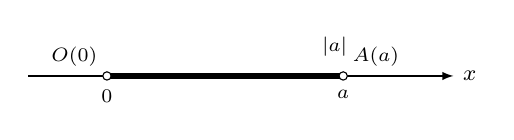
\begin{tikzpicture}
\draw[-latex] (-1,0) -- coordinate (x axis mid) (4.4,0) node[right,fill=white] {{\footnotesize $ x $}};
\draw (0,.5mm) -- (0,-.5mm) node[anchor=north,fill=white] {{\scriptsize $ 0 $}};
\draw (3,.5mm) -- (3,-.5mm) node[anchor=north,fill=white] {{\scriptsize $ a $}};
\draw[line width=.7mm] (0,0) -- (3,0);
\tkzText(1.5,.34){$ \overcbrace{\rule{28mm}{0mm}}^{{\scriptsize |a|}} $}
\tkzDefPoint(3,0){A}
\tkzDrawPoint[size=3,fill=white](A)
\tkzLabelPoint[above right](A){{\scriptsize $A(a)$}}
\tkzDrawPoint[size=3,fill=white](0,0)
\tkzLabelPoint[above left](0,0){{\scriptsize $O(0)$}}
\end{tikzpicture}
\end{tabular} 
\end{center}
\begin{itemize}[itemsep=0mm]
\item Απόσταση δύο αριθμών $a$ και $\beta$
\[ |a-\beta|=d(a,\beta) \]
\end{itemize}
\begin{center}
\begin{tabular}{c >{\centering\arraybackslash}m{6cm}}
$ |a-\beta|=d(a,\beta) $  & 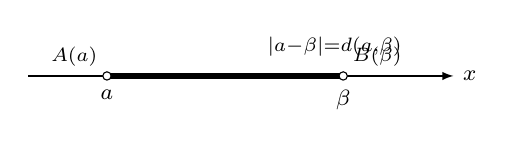
\begin{tikzpicture}
\draw[-latex] (-1,0) -- coordinate (x axis mid) (4.4,0) node[right,fill=white] {{\footnotesize $ x $}};
\draw (0,.5mm) -- (0,-.5mm) node[anchor=north,fill=white] {{\footnotesize $ a $}};
\draw (3,.5mm) -- (3,-.5mm) node[anchor=north,fill=white] {{\footnotesize $ \beta $}};
\draw[line width=.7mm] (0,0) -- (3,0);
\tkzText(1.5,.34){$ \overcbrace{\rule{28mm}{0mm}}^{{\scriptsize |a-\beta|=d(a,\beta)}} $}
\tkzDefPoint(3,0){A}
\tkzDrawPoint[size=3,fill=white](A)
\tkzDrawPoint[size=3,fill=white](0,0)
\tkzLabelPoint[above right](A){{\scriptsize $B(\beta)$}}
\tkzLabelPoint[above left](0,0){{\scriptsize $A(a)$}}
\end{tikzpicture}
\end{tabular} 
\end{center}
\kerkissans{Ιδιότητες απόλυτων τιμών}\\
Για κάθε $ a,\beta\in\mathbb{R} $:
\begin{itemize}[label=\faCheckCircle]
\item $ |a|=|-a|\geq0 $
\item $ |a|=0\Leftrightarrow a=0 $
\item $ -|a|\leq a\leq|a| $
\item $ |a\cdot\beta|=|a|\cdot|\beta| $ 
\item $ \left| \dfrac{a}{\beta}\right|=\dfrac{|a|}{|\beta|} $ 
\item $ |a|^2=a^2 $
\item $ \left||a-\beta| \right|\leq|a\pm\beta|\leq|a|+|\beta|  $ 
\end{itemize}
\begin{itemize}[label=\faStop]
\item $|x-x_0|<\rho\Leftrightarrow x_0-\rho<x<x_0+\rho$ ή $x\in(x_0-\rho,x_0+\rho)$
\item $|x-x_0|>\rho\Leftrightarrow x<x_0-\rho\ \ \text{ή}\ \ x>x_0+\rho$ ή $x\in(-\infty,x_0-\rho)\cup(x_0+\rho,+\infty)$
\end{itemize}
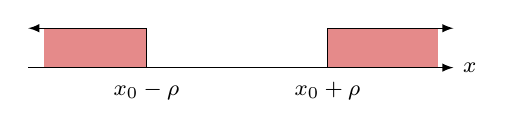
\begin{tikzpicture}
\fill[red7] (0.5,0) rectangle (-0.8,0.5);
\fill[red7] (2.8,0) rectangle (4.2,0.5);
\draw[-latex] (0.5,0)--(0.5,0.5)--(-1,0.5);
\draw[-latex] (2.8,0)--(2.8,0.5)--(4.4,0.5);
\draw[-latex] (-1,0) -- coordinate (x axis mid) (4.4,0) node[right,fill=white] {{\footnotesize $ x $}};
\node at (0.5,-0.3){\footnotesize$x_0-\rho$};\\
\node at (2.8,-0.3){\footnotesize$x_0+\rho$};
\end{tikzpicture}
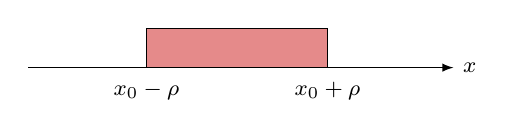
\begin{tikzpicture}
\fill[red7] (0.5,0) rectangle (2.8,0.5);
\draw[-] (0.5,0)--(0.5,0.5)--(2.8,0.5)--(2.8,0);
\draw[-latex] (-1,0) -- coordinate (x axis mid) (4.4,0) node[right,fill=white] {{\footnotesize $ x $}};
\node at (0.5,-0.3){\footnotesize$x_0-\rho$};\\
\node at (2.8,-0.3){\footnotesize$x_0+\rho$};
\end{tikzpicture}
\end{document}